\section{Analysis} \label{sec:Analysis}

\subsubsection{Calibrated Model}

\begin{table}[H]
\center
\begin{threeparttable}[b]
\caption{Parameters of the model}
\label{tab:ModelCalib}
\begin{tabular}{@{}ll@{\hspace{1.5cm}}ll@{}}
\toprule
 & Parameter                              & Notation         & Value    \\ \midrule 
\multicolumn{4}{l}{\textit{Calibrated}}                                 \\
 & Mean consumption growth                & $g$              & $0.0134$ \\
 & Standard deviation of $\Delta c_t$     & $\sigma$         & $0.0152$ \\
 & Standard deviation of $\Delta d_t$     & $\sigma_w$       & $0.1256$ \\
 & Log risk-free rate                     & $r^f$            & $0.0109$ \\
 & Persistence parameter                  & $\phi$           & $0.9008$ \\
 \multicolumn{4}{l}{\textit{Assumed}}                                   \\
 & Coefficient of Risk Aversion           & $\gamma$         & $2.0000$ \\
 & Correlation dividends/consumption      & $\rho$           & $0.2000$ \\
\multicolumn{4}{l}{\textit{Implied}}                                    \\
 & Subjective discount factor             & $\delta$         & $0.9156$ \\
 & Steady-state surplus consumption ratio & $\Bar{S}$        & $0.0666$ \\
 & Maximum surplus consumption ratio      & $S_{\text{max}}$ & $0.1096$ \\ \bottomrule
\end{tabular}
\begin{tablenotes}
\footnotesize{\item [1] All relevant parameters are annualized
              \item [2] Calibrated parameters are estimated from data, assumed are chosen arbitrarily on the grounds of existing literature, while implied parameters are calculated from the calibrated/assumed parameters.}
\end{tablenotes}
\end{threeparttable}
\end{table}

%\begin{table}[H]
\centering
\begin{threeparttable}[b]
\caption{Parameters of the model}
\label{tab:ModelCalib}
\begin{tabular}{@{}ll@{\hspace{1.5cm}}ll@{}}
\toprule
 & Parameter                              & Notation         & Value    \\ \midrule
\multicolumn{4}{l}{\textit{Calibrated}}                                 \\
 & Mean consumption growth                & $g$            & $0.0134$ \\
 & Standard deviation of $\Delta c_t$     & $\sigma$         & $0.0152$ \\
 & Standard deviation of $\Delta d_t$     & $\sigma_w$       & $0.1256$ \\
 & Log risk-free rate                     & $r^f$            & $0.0109$ \\
 & Persistence parameter                  & $\phi$           & $0.9008$ \\
 \multicolumn{4}{l}{\textit{Assumed}}                                   \\
 & Coefficient of Risk Aversion           & $\gamma$         & $2$ \\
 & Correlation dividends/consumption      & $\rho$           & $0.2$ \\
\multicolumn{4}{l}{\textit{Implied}}                                    \\
 & Subjective discount factor             & $\delta$         & $0.9156$ \\
& Steady-state surplus consumption ratio & $\Bar{S}$        & $0.0666$ \\
 & Maximum surplus consumption ratio      & $S_{\text{max}}$ & $0.1096$ \\ \bottomrule
\end{tabular}
\begin{tablenotes}
\footnotesize{\item [1] All relevant parameters are annualized
              \item [2] Calibrated parameters are estimated from data, assumed are chosen arbitrarily on the grounds of existing literature, while implied parameters are calculated from the calibrated/assumed parameters.}
              
\end{tablenotes}
\end{threeparttable}
\end{table}
\begin{table}[H]
\centering
\begin{threeparttable}[b]
\caption{Parameters of the model}
\label{tab:ModelCalib}
\begin{tabular}{@{}ll@{\hspace{1.5cm}}ll@{}}
\toprule
 & Parameter                              & Notation         & Value    \\ \midrule
\multicolumn{4}{l}{\textit{Calibrated}}                                 \\
 & Mean consumption growth                & $g$            & $0.0134$ \\
 & Standard deviation of $\Delta c_t$     & $\sigma$         & $0.0152$ \\
 & Standard deviation of $\Delta d_t$     & $\sigma_w$       & $0.1256$ \\
 & Log risk-free rate                     & $r^f$            & $0.0109$ \\
 & Persistence parameter                  & $\phi$           & $0.9008$ \\
 \multicolumn{4}{l}{\textit{Assumed}}                                   \\
 & Coefficient of Risk Aversion           & $\gamma$         & $2$ \\
 & Correlation dividends/consumption      & $\rho$           & $0.2$ \\
\multicolumn{4}{l}{\textit{Implied}}                                    \\
 & Subjective discount factor             & $\delta$         & $0.9156$ \\
& Steady-state surplus consumption ratio & $\Bar{S}$        & $0.0666$ \\
 & Maximum surplus consumption ratio      & $S_{\text{max}}$ & $0.1096$ \\ \bottomrule
\end{tabular}
\begin{tablenotes}
\footnotesize{\item [1] All relevant parameters are annualized
              \item [2] Calibrated parameters are estimated from data, assumed are chosen arbitrarily on the grounds of existing literature, while implied parameters are calculated from the calibrated/assumed parameters.}
\end{tablenotes}
\end{threeparttable}
\end{table}



Compared to the calibration of \citet{Campbell1999}, our calibration suggests a higher persistence parameter, higher volatility of dividend growth and lower consumption growth, the implied surplus consumption parameters suggests a slightly higher overall surplus consumption. The differences likely stems from the extra 20 years of calibration data. \\
\subsection{Simulation}
From the calibrated model we simulate a chain of 100.000 monthly draws from the economy yielding 8.332 years of simulated time-series. Allowing us to infer about the predictability of excess stock returns, during times of simulated crisis. \\
\newline
Based upon NCER-recession data, we find that the US economy was in recession approximately 13.4\% of the period spanning January 1950 until December 2018.  In the model a recession implies that present consumption in low relative to previous periods consumption, that is the value of $s_t$ is lower than the steady state value of surplus consumption $\Bar{s}$ - integrating over the density of $s_t$ yields that the simulated economy is in recession during 37\% of all observations, which indicates that $\Bar{s}$ might be misspecified. To correct $\Bar{s}$ we match the empirical business cycle behavior by numerical optimization of the $s_t$ density, such that the empirical and simulated economy is in recession roughly the same amount. The $\Bar{s}$-value matching the empirical business cycle, throughout denoted $\Bar{s}_{rec}$ \textit{or} ($\Bar{S}_{rec}$), is found to be $-3.18$ ($0.0415$).

\begin{figure}[H]
    \centering
    \caption{Distribution of simulated $s_t$ chain}
    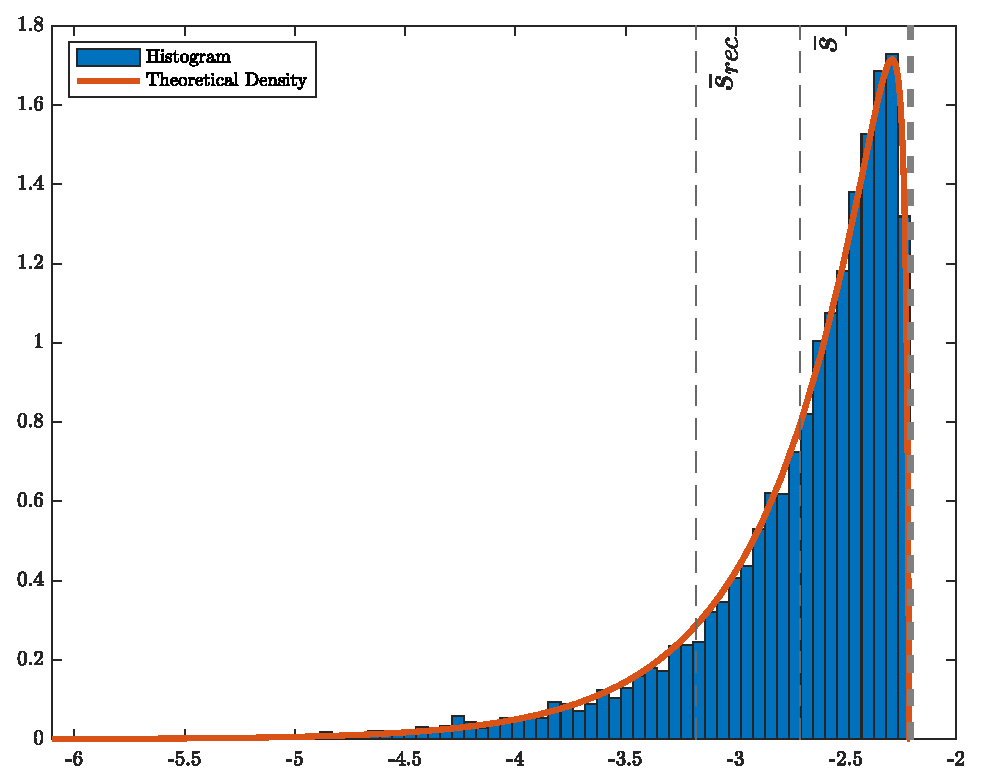
\includegraphics[width=\textwidth]{Figures/DistributionS_t.eps}
    \label{fig:DistriSt}
\end{figure}

\begin{table}[H]
\centering
\caption{Data Properties}
\label{tab:Data_props}
\begin{tabular}{@{}l@{\hspace{1.5cm}}l@{\hspace{1.5cm}}l@{}}
\toprule
 & \textit{Simulated} & \textit{Historic} \\ \midrule
$\mathbb{E}\left[r_t- r^f_t\right]$& $0.0373$           & $0.0927$          \\
$\sigma\left(r_t - r^f_t  \right)$ & $0.0962$           & $0.1670$          \\
$\mathbb{E}\left[r_t- r^f_t\right] / \sigma\left(r_t - r^f_t,\right)$ & $0.3877$ & $0.5548$  \\ \bottomrule
\end{tabular}
\end{table}

%\begin{table}[H]
\centering
\caption{Data Properties}
\label{tab:Data_props}
\begin{tabular}{@{}l@{\hspace{1.5cm}}l@{\hspace{1.5cm}}l@{}}
\toprule
 & \textit{Simulated} & \textit{Historic} \\ \midrule
$\mathbb{E}\left[r_t- r^f_t\right]$& $0.056558$           & $0.0927$          \\
$\sigma\left(r_t - r^f_t  \right)$ & $0.16886$           & $0.167$          \\
$\mathbb{E}\left[r_t- r^f_t\right] / \sigma\left(r_t - r^f_t,\right)$ & $0.33493$ & $0.5548$  \\ \bottomrule
\end{tabular}
\end{table}

\subsection{Simulated}

\begin{table}[H]
\centering
\caption{Simulated Moments}
\label{tab:MMoomme}
\begin{tabular}{@{}llllllllll@{}}
\toprule 
 & $\mathbb{E}\Delta d$ & $\sigma_{\Delta d}$ & $\mathbb{E}r^f$ & $\mathbb{E}r^m/\sigma _{r^m}$ & $\mathbb{E}R^m/\sigma _{R^m}$ & $\mathbb{E}r^m$ & $\sigma_{r^m}$ & $\mathbb{E}d-p$ & $\sigma_{d-p}$  \\ 
\midrule 
\multicolumn{10}{l}{$P/D$}\\
 &0.011661&0.10257& 0.010881 & 0.21595 & 0.28775 & 0.0354 & 0.16393 & 3.3797 & 0.1864 \\ 
\multicolumn{10}{l}{$P/C$}\\
 &0.013504&0.01243& 0.010881 & 0.38534 & 0.42038 & 0.037242 & 0.096645 & 3.3797 & 0.1864 \\ 
\bottomrule 
\end{tabular}

\end{table}

%\input{Code_v2/Tables/Table_3.tex}

\begin{table}[H]
\centering   
  \caption{Regressions}           
  \label{tab:regress}     
  \begin{threeparttable}
\begin{tabular}{@{\hspace{5pt}}l@{\hspace{5pt}}cccc} 
\toprule 
 & \multicolumn{4}{c}{\textit{Dependent variable:}} \\ 
 & \multicolumn{4}{c}{$\left(r_{t+1}-r^f\right)$} \\ 
 \cmidrule(rr){2-5}
 & (1)   &   (2) &   (3) &  (4)\\ 
\midrule  
\\[-2.1ex] $\left( p_t - c_t \right)_{REC}$ & $-$0.169& &  \\ 
  & (0.012) & & & \\ 
 \addlinespace 
  $\left( p_t - c_t \right)_{EXP}$ & $-$0.1641 & &  \\ 
  & (0.0098) & & &\\ 
 \addlinespace 
 $p_t - c_t$ &  & $-$0.1516 & & \\
 & & (0.0071) \\
 \addlinespace 
  $\left( p_t - d_t \right)_{REC}$ & & & $-$0.1719&  \\ 
  & & & (0.016)    &\\ 
 \addlinespace 
  $\left( p_t - d_t \right)_{EXP}$ & & & $-$0.1668&  \\ 
  &  & & (0.012) &\\ 
 \addlinespace 
 $p_t - d_t$ & & & & $-$0.1552 \\
 & & & &  (0.0086)  \\
 \addlinespace 
 Constant &0.5611 &0.5206 &0.5736 &0.5352 \\ 
  &(0.032) &(0.023) &(0.041) &(0.028) \\ 
 \addlinespace 
\midrule  
Observations & 8331 & 8331 & 8331 &8331\\ 
R$^{2}$ &0.094 & 0.094 & 0.053 &0.052\\ 
Residual Std. Error &0.015 & 0.015 &0.037 & 0.037  \\ 
\bottomrule 
\end{tabular} 
\begin{tablenotes}
\footnotesize{
\item[1] Brackets below estimates contains Newey-West corrected standard errors. 
\item[2] Regressions on 8331 years of simulated data.
\item[3] EXP (REC) denotes expansion (recession)
}
\end{tablenotes}
\end{threeparttable}
\end{table} 

\begin{table}[H]
\centering   
  \caption{Regime Switching Regression}           
  \label{tab:RSregress}     
  \begin{threeparttable}
\begin{tabular}{@{\hspace{5pt}}l@{\hspace{5pt}}cccc} 
\toprule 
 & \multicolumn{4}{c}{\textit{Dependent variable:}} \\ 
 & \multicolumn{2}{c}{$\left(r_{t+1}-r^f\right)_{REC}$} & \multicolumn{2}{c}{$\left(r_{t+1}-r^f\right)_{EXP}$} \\ 
 \cmidrule(rr){2-5}
 & (1)   &   (2) & (3) & (4) \\ 
\midrule  
\\[-2.1ex] $ p_t - c_t $ & 0.02183&  &-0.01055   & \\ 
  & (0.0019) & &(0.0013) & \\ 
 \addlinespace 
 $p_t - d_t$ &  & 0.02192 & &-0.01429 \\
 & & (0.0025) & &(0.00159) \\
 \addlinespace 
 Constant &-0.004529 &-0.005873 &0.07522 &0.08416 \\ 
  &(0.00044) &(0.00061) &(0.004) &(0.0048) \\ 
 \addlinespace 
\midrule  
Observations & 8331 & 8331 & 8331 &8331\\ 
R$^{2}$ &0.068 & 0.04 & 0.011 &0.0084\\ 
Residual Std. Error &0.005 & 0.0088 &0.012 & 0.029  \\ 
\bottomrule 
\end{tabular} 
\begin{tablenotes}
\footnotesize{
\item[1] Brackets below estimates contains Newey-West corrected standard errors. 
\item[2] Regressions on 8331 years of simulated data.
\item[3] EXP (REC) denotes expansion (recession)
}
\end{tablenotes}
\end{threeparttable}
\end{table} 
